% This file is based on the "sig-alternate.tex" V1.9 April 2009
% This file should be compiled with V2.4 of "sig-alternate.cls" April 2009

\documentclass{sig-alternate}

\usepackage{graphicx}
\usepackage{url}
\usepackage{color}
\usepackage{enumerate}
\usepackage{balance}
\permission{}
\CopyrightYear{2013}

\usepackage[english]{babel}
\usepackage{blindtext}

\usepackage{etoolbox}
\makeatletter
\patchcmd{\maketitle}{\@copyrightspace}{}{}{}
\makeatother

%\crdata{0-00000-00-0/00/00}
\begin{document}

%%% Maketitle 
\newcommand{\horrule}[1]{\rule{\linewidth}{#1}} 	
% Horizontal rule

\title{
		%\vspace{-1in} 	
		\usefont{OT1}{bch}{b}{n}
		\normalfont\normalsize 
		\textsc{Rochester Institute of Technology}	\\ [25pt]
		\horrule{0.5pt} 								\\[0.4cm]
		\huge What Should I Wear 					\\
		\horrule{2pt} 								\\[0.5cm]
		\vspace{-10mm}
}

\author{
		\normalfont\normalsize 
        Piter Garcia and Anthony Castiglia			\\[-3pt]
        	\normalsize\today
}
\date{}
\maketitle

\begin{abstract}

	The aim of this project is to implement some cleaning and mining techniques that we have learnt in a 	project chosen by our team. The name of our project is "What Should I Wear," and we will be using 		weather data sets of the United States to analyze, compare, and approximate the weather trends 			including the precipitation of a particular area requested by the user in a designated input time 		range. In fact, we will be able to suggest users whether they should wear a coat or not through an 	interface that we have designed to allow users to consult what to wear according to the weather of 		the city, including its precipitation, for short-term travel or vacation purpose.
\end{abstract}
\vspace{5 mm}

\section{Overview}
	\label{overview}

	The logical structure of our project is composed of three main phases that better describe the 			milestones achieved throughout our project development. These phases are classified as Design, 			Architecture and Implementation. Each phase explains in detail the main steps taken to model and 			structure a database with our interface to meet the project specifications. In order to better 			organize our documentation we have divided these phases into two main sections that contain a 			summary of the work process done in our project. These two sections are Database and Interface, and 		their development can be described as follows:\newline

	In the database,the datasets consist of maximum and minimum temperature, precipitation, wind speed, 		longitude and latitude (position about 1/8 degrees apart) of some locations. These datasets have 			been collecting weather information for the past forty four years. This amount of data helps us 			analyze the trends of some areas over the past years, and makes our results more reliable. The main 		goal was to design a database, from which we can easily generate tables for the cities, cities' 			weather 	information, and user' s cities selections.\newline
    
	In the interface, the design works as a platform to shape and implement our project according to our 	expectations. The way we have designed our interface is according to the database design. Therefore, 	we have created a set of features that users will be able to use in a website through our database 		implantation. The appearance of our website is highly influenced by the architecture of our project, 	and even though our first interface design appearance may not correlate with the implementation, the 	features are the same. We used certain tools in order to provide our interface with the structure 		needed to meet our project specifications. For this project, App Engine NDB datastore is the 				database engine 	underlined by our management system to create, read, update and delete data from the 	database. Moreover, we have included other database and web development software that have helped us 	model and process our database faster and easier. The application programming interface that we are 		using, to allow users to interact with our underlying engine without going through our system, is 		webapp2. We are also making use of tools such as Python and HTML. \newline

	In particular, we will explain some tools and techniques used to achieve our goals in each one of 		the sub-sections explained in the Database and Interface sections. These subsections are explained 		separately in each sub-structure as the process taken in each one varied. Our main goal is to make 		querying for the weather information easy and reliable. This can be accomplished through our 				database and interface application by taking the input of users and providing them with a graphical 		output that can be easily interpreted.\newline

\section{Design}
	\label{Design}

	\textbf{Figure 1: Example Design}\newline
	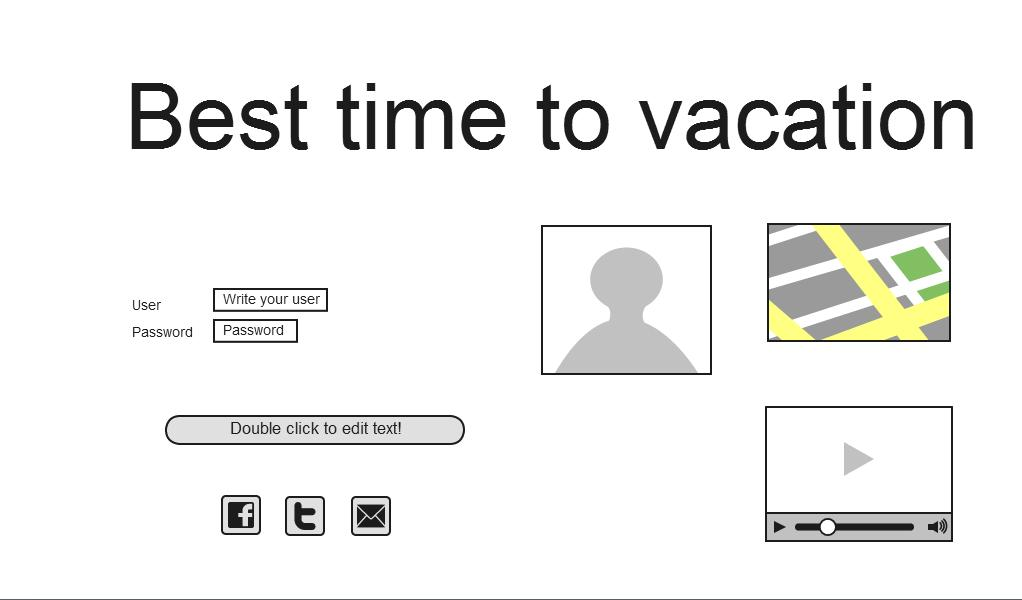
\includegraphics[scale=0.2]{design.eps} 
	
	The operational process of our design meets the objective of a high quality development which 			responds to real life scenarios in big data. The focus of this step is the development of an 				acceptable functional solution to the requirements of our project with an exterior design solution 		that is compatible with our database, interface, and our goal as a whole. A successful design 			development is needed in order to coordinate the activities of users and project architecture to 			meet our goal.
	\newline

	\subsection{Database}

		We are using data sets provided by the University of Washington's Surface Water Modelling 				Group. The data sets contain daily and monthly records of daily total precipitation, maximum 				temperature, minimum temperature, and average 10-meter wind speed. The data is available both 			per-month and per-day for fifteen regions in North America. Data is available for all regions 			for dates ranging from 1949 to 2000, as well as earlier and later for some regions. This project 		will be focusing on the data that is available for all regions (from 1949 to 2000). \newline

		\textbf{Figure 2: Example Data Table Design}\newline
		
\includegraphics[scale=0.215]{table.eps} 
		\begin{description}
  			\item[Preparation] \hfill \\
				The main goal was to make querying for the weather information easy and reliable. 						Therefore, to make a better use of the database, we have formatted each dataset to 						remove redundant, noisy, and unnecessary data, which helped our system to run more 						efficiently.\newline  

				The main purpose of the preparation process was to make our database look as Figures 						3,4,5 and 6. In this way, we are able to read the formatted data files according to the 					requirements of our project. This process allows us to easily relate each one of the 						input dates to the corresponding city and its temperature, within the given range, to 					approximate the weather condition of the city within the given dates.  \newline

				In order to create the desired appearance described above, we needed to make our 							database go through some steps to make this structure possible. 
				
				\begin{itemize}
  					\item First, the datasets were compressed and therefore we needed to extract them 							by using the little Edian format, which was a very difficult process to include 						in our code. 
  					
  					\item Second, we sorted the cities and separated them from those we did not plan to 							include in our database. Also, the datasets were huge and unnecessary for our 							implementation. Therefore, we modified the datasets to contain only weather 								information from 1980 to 2000. This, based on the resulting data, includes 								enough data for the purpose of our project.

  					\item Lastly, each dataset was formatted to relate to the weather, user, and 									longitude-and-latitude tables to its corresponding city by means of an id, 								which enabled us to match a city weather records' dates to the user given 								dates.
				\end{itemize}

				The datasets we obtained were huge and very difficult to handle. The preparing process 					was a very important step in our project to improve and speed up every process. At 						first, it was very difficult for us to test our features because the system was slow and 				overloaded with data. This is why we proceeded to exclude a large amount of cities and 					only work with some cities to make testing more efficient and reliable.

  			\item[Cleaning] \hfill \\
  				We designed the database appearance and structure to perform according to the results of 				our cleaning process. The purpose was to allow the tables in our database to 	relate to 					the input dates, corresponding city and its temperature. Thus, we would be able to 						approximate the city' s weather condition within the given range of the input dates in 					an easier and faster manner.  Our main model was based on the Temperature, City Tables, 					and their structure was studied by tools that are explained in the architecture phase of 				this project. An example of the design of these tables' structures can be seen in the 					Figures 5 and 6. User's table was designed, but it is supposed to have a different 						structure to the others since this table is populated as users register.\newline

				After the user access our system, the content of this will access the other tables 						such as the city and weather tables. Once it has gathered the necessary data it will 						proceed to do some data processing techniques, explained in the implementation phase, to 				approximate the weather condition of a city selected by the user within the input dates. 				This performance is explained in details in the architecture phase of this project.						\newline
				
				\textbf{Figure 3: City Entry Design}\newline
				
\includegraphics[scale=0.5]{cities.eps} 
				
				\textbf{Figure 4: Data Entry Design}\newline
				
\includegraphics[scale=0.4]{data.eps} 					
				The main tables used to create our database are the Data and City tables. These tables 					were created, after uncompressing the data, with an algorithm we coded in Java. This 						process 	is explained in detail in the architecture phase; we will briefly explain how 					the design of this process took place.\newline
				
				\textbf{Figure 5: City Table Design}\newline
				
\includegraphics[scale=0.5]{cityT.eps}
				 	
				In order to load our tables into our system it was necessary for us to have the two 						tables, mentioned above, formatted.\newline

				\textbf{Figure 6: Data Table Design}\newline
				
\includegraphics[scale=0.5]{dataT.eps} 		
				
				The structure of each table should be as follows. First, the City table, this is 							composed by latitude, longitude, and the cityName. Lastly, the Data table, which is 						composed by the date, precipitation, temperature, and wind of each city. This is the 						structure we used to design our database as shown in the Figures 5 and 6. The Data 						tables must be used by our interface to implement the features of our system. This 						includes weather approximation as well as to suggest cities that the user may like 						according to the user's behavior, which has not been implemented yet.

		\end{description}

	
	\subsection*{Interface} 
		We have designed a website that works as a platform to shape and implement our project according 		to our expectations and database design. We have created a set of features that users are able 			to use in our website through our database and code implementation.\newline
		
		\textbf{Figure 7: Interface Structure Design}\newline
		\includegraphics[scale=0.2]{design2.eps} 
		
		An example of the appearance of our interface frame design is in Figure 7. Our website is highly 		influenced by the architecture of our project, and therefore its design may not look exactly, or 		even similar, to the original result.\newline\newline\newline\newline
		
		\textbf{Figure 8: Search Place Design}\newline
		
\includegraphics[scale=0.27]{search.eps} 
		We used certain tools in order to provide our interface with the structure needed to meet our 			project specifications. For this project, "App Engine NDB datastore" is the database engine 				underlined by our management system to create, read, update and delete data from the database. 			Moreover, we included other database and web development software that helped us model and 				process our 	database faster and easier. The application programming interface that we are using, 		to allow users to interact with our underlying engine without going through the user interface 			of our system, is webapp2. We are also making use of tools such as Python and HTML. These tools 			are 	described in detail in the architecture section of our project, and examples of these are 			given to show the reader how the structure design of our interface took place.\newline

		The platform that we are using to manage our database is webapp2. The installation and upgrading 		process is very easy since we have the ability to automatically install database adapters and 			other dependencies. Using webapp2 in our management systems allow us to extract valued 					content from our datasets and build a high performing web applications system in an elegant and 			efficient way. The following factors improve with the use of webapp2. \newline

		\begin{itemize}
  			\item First, we can define our data models much easier with Python that provides us with a 				dynamic 	database access APIA that has been formatted with SQL. 
  			
  			\item Second, it provides an automatic admin interface that adds and updates users and 					user's content automatically. 
  			
  			\item Third, it supports Multi-language applications. This is essential for our 							implementation since it is used for travelling, especially vacation purposes. 
  			
  			\item Finally, we can always use cache frameworks to increase future performance.
		\end{itemize}		
		
		All features of our project were designed to help users to decide what they should wear when 				travelling and, or, going on vacation. In order to achieve this, we need to provide users with 			features that allow them to search for a place, monitor the approximate weather information, and 		have a list of suggested cities that users may want to visit accordingly. The design of these 			features can be described as follows:\newline

		The idea is to have a system in which we  assign each user with a unique id and password. An 				example of this feature can be seen in the Figure 7, but this is not fully implemented in our 			system yet. Because of the time we are only proving with clothing suggestions. We have an 				application for users to access our system through a website, and to facilitate users to utilize 		it in a more efficient manner we need to improve our system as follows.\newline

		\begin{itemize}
  			\item First, incorporate and increase user registrations quickly. 
  			\item Second, provide users with an app id and app secret-id; this has not been implemented 				yet. 				
  			\item Overall, these features could potentially help us integrate more features and allow 				for 	future improvements.
		\end{itemize}
		
		\textbf{Figure 9: Search Place Table Design}\newline
		
\includegraphics[scale=0.4]{searchT.eps} 
		
		We did not implement this feature, however, this feature would have allowed users to personally 			search and find cities of their interest. This feature would automatically add the searches done 		by the user; the list of searches or table would provide suggestions to the user with a list of 			cities that he or she may like. More detail of the structure of this feature is covered in the 			architecture phase of our project. The image in Figure 9 is an example of this feature's design.			\newline
 		
 		\textbf{Graph}\newline
		In the graph feature, there is a function that we use to approximate the weather information of 			a city. Once the weather data was approximated, this data is accessed and analyzed for the 				system to provide the user with a clothing suggestion. The process in which we make use of the 			weather data to make the approximation is better explained throughout our project.\newline
 
		\textbf{Suggestion List}\newline
		This feature was not implemented, but it would have shown a graphical representation of the 				approximated weather and precipitation of the designated city that the user searched for. We 				would have used the table that stores all the searches done by the user, and use the data in 				this table such as user's information and the weather information of the cities. After all this 			information was gathered, we would have created another table to contain the suggested cities 			that the user may want to visit. \newline
		
\section{Architecture}
	\label{architecture}

	It was critical to model the right architecture in order to succeed in our system and implementation 	design. The architecture process is an essential part of our project, which specifies the overall 		structure of our system. In this process with provide you with the description and analysis of high 		level properties of our system originated from our database and interface. The database contains the 	assignment of functionality for our designed features, data corporal distribution, composition of 		designed features, scaling and performance, and data design modifications. In contrast, the 				interface section includes the body of work for our module interconnection features, templates and 		frameworks for our system that serve the needs of our database domain, and formal models of 				component integration mechanisms. \newline
	
	\subsection*{Database}
	
	\begin{description}
		\item[Preparation] \hfill \\

			In the formatting process of our project we used some algorithm techniques to model our data 			to meet the project requirements. The appearance of the database was obtained through 					algorithms such as the little EDIAN. Also, we used our own Java code implementation to 					reduce the datasets to only 20 years of weather information, and to reduce the number of 					cities. \newline
			
			\textbf{Figure 10: Little Edian Script}\newline
			
\includegraphics[scale=0.2]{IDEAN.eps} 
			\newline 
			
			Little EDIAN is a compression format algorithm that we used to uncompress the datasets 					mentioned in the design section of our project. We had access to the algorithm through 					Washington University Website referenced below, and a demonstration of the algorithm is 					shown in Figure 10.\newline
			
			\textbf{Figure 11: Reduction Data JAVA}\newline
			
\includegraphics[scale=0.2]{JCL1.eps} 
			\newline 
			
			We implemented in JAVA the code shown in Figure 11. This code reduces the data to 20 years 				of weather information, and it loads the datasets from 15 different territories.\newline

			In order to use our database, we had to model each dataset to load and query easily. To do 				this, we have used our own code implementation that creates the city and data table 						explained in the designed section. These tables are created by the algorithm shown in the 				Figure 11. This algorithm Figure 11: Java Source Code - Reduction Data consist of two parts; 			the first is creating the city table and the second is creating the data table. An image of 				these two is shown in the Figures 5 and 6.\newline
 
			The reduction and formatting of the datasets made easier the querying process. The algorithm 			mentioned in the structure of this division was necessary in order to perform our testing 				procedures. The reason for this is because the datasets were huge, and we did not need more 				than 20 years of weather data to approximate the weather of a city.\newline


		\item[Cleaning] \hfill \\
	
			The structure of our database was modelled through the pgAdminIII work platform. This work 				platform helped us to generate the tables that we needed to make possible the 							functionalities of each features. Through this application we were able to generate the city 			and data tables, which are very essential for our implementation. A demonstration of the 					work platform is shown in the Figure 12.\newline
 
			The structure of the pgAdmingIII platform devises a query plan for each query that is given 				to generate the tables. The generation of these tables will decrees the querying time, and 				gives us a close approximation in a quick step.\newline
			
			\textbf{Figure 12: Work Platform}\newline
			
\includegraphics[scale=0.3]{platform.eps} 
			\newline

			The data table consist of weather information of the cities, these are temperature maximum 				and minimum, precipitation and wind speed. These weather information corresponds to each 					city id, and the data is from 1980 to 2000. The schema of this table is shown in the image 				above. City, the data table for the city, contains only the id, the longitude, and latitude 				of each city. The id is used as a reference to the Data table. The schema of this is shown 				in the Figure 14.\newline

			\textbf{Figure 13: User Profile Table}\newline
			
\includegraphics[scale=0.4]{userP.eps} 					
			\textbf{User}\newline
			We are not currently implementing this table in our interface because we ran out of time. 				However,  this table can be used in the pgAdminIII work platform to query accordingly in 					future.\newline
 
 			\textbf{Figure 14: City Data Structure}\newline
 			
\includegraphics[scale=0.4]{cityD.eps} 
			\textbf{City Data}\newline
			Contains the data of temperature, wind, precipitation that matches with the cities.\newline
			
			\textbf{Figure 15: City Search Structure}\newline
 			
\includegraphics[scale=0.4]{cityS.eps} 
		
			Contains the data of temperature, wind, precipitation that matches with the cities.\newline
		
			\textbf{Search}\newline
			In the search place table, we have assigned this to each area. Then, we named it city in our           			query, a unique id through which we can distinguish it from the other areas. \newline
	
	\end{description}
	
	\subsection*{Interface}
	
		The structure of our interface is modelled by webapp2, and other alternatives, through its 				queries techniques. We used 	these techniques to populate the user table, to query the other 				tables in our database, and to perform some data mining techniques. webapp2 provides for an 				intuitive way of representing the database in python. It uses a model class for database tables 			where an instance of a class represents a record of each table, as shown in the image below.				\newline 
		
		\textbf{Figure 16: Work Platform 2}\newline
	 	
\includegraphics[scale=0.1]{platform2.eps} \newline
	 	
	 	An example of our interface development is shown in the Figure 7. The features that we display
		are search, graph, and clothing suggestions. The design structure of each of these is covered 			below.\newline
	
		\textbf{Figure 17: Work Platform 3}\newline
		
\includegraphics[scale=0.1]{platform3.eps} \newline

		\textbf{Creating Objects}\newline
		To create an object, we would need to instantiate this class using keywords to model class, and 			then save the changes. The class needs to be imported using the python path to the class. 				Assuming models live in a le mysite = blog = models.py, The code in Figure 16 adds a record to 			Blog().\newline

		\textbf{Updating Objects}\newline
		This is an intuitive task where we perform the updating in the class. Next, we ask the database 			to save the changes. The example in Figure 17 changes the name of the instance of the class to 			b5.\newline

		\textbf{Retrieving Objects}\newline
		This is done using the Queryset on the manager. Queryset in Django is equivalent to a select 				statement. In the example below, the object represents the default manager and Blog() represents 		the query set with a few filters that filter out the results. Next, a number of filters can be 			used on the resultant query. Keywords like filter and exclude are used for that. The keyword 				"all" is used if all the results are required. In case we require only a single output the 				keyword get is used. We could also limit the results such that we get a range of results from 			the table.\newline

		\textbf{Person Objects}\newline
		The table Person has not been implemented in our interface yet, but is very necessary when 				implementing the algorithm to obtain a list of suggested cities that users may like. All the 				data gathered is saved in a table named Person, and the reason why is important is because this 			table would allows us to identify users and predict users' behavior according to their search 			history.\newline

		Overall, the architecture of our system can be improved by understanding the complexity of our 			system. We still are recognizing common paradigms that allow high level relationships among 				systems to be understood, and we will be able to build a new system as variations on our 					current systems.
		\vspace{-4mm} 
			
\section{Implementation}
	\label{implementation}

	The Implementation section describes how system applications will be installed, deployed and 				transitioned into our operational system for the purpose of our project. In this section we will 			provide you with an overview of the system, describe major tasks involved in the implementation 			process, and the overall resources needed to support the implementation effort such as hardware, 			software, facilities, techniques, among others. Furthermore, we will present users with the 				documentation and tools necessary to make an informed decision on how to deploy our system for 			short-term travelling cloth wearing suggestions. In addition, multiple features have been added and 		we will explain how to utilize them in our system during its implementation process. We will 				demonstrate how these applications, based on our interface and database sections, can be installed 		and configured in any environment by deploying the enabled operations of our system that have been 		completely developed and tested for our project.

	\subsection*{Database}
		\begin{description}
  			\item[Preparation] \hfill \\
  				\textbf{Database Reduction}\newline
					We have reduced the amount of data we have, obtained from the online source cited 						below, due to our current design. We did not believe that more than 20 years of data 					was necessary to achieve the goal of this project. And since the cleaning and 							preparation process of the data was taking too long because of the data sets being 						too big, our computer processors were having trouble to handle our database. The two 					images is a comparison between our database before and after shrinking the data sets 					to 20 years of data.
					
					\textbf{Figure 18: Original Database Scale}\newline
					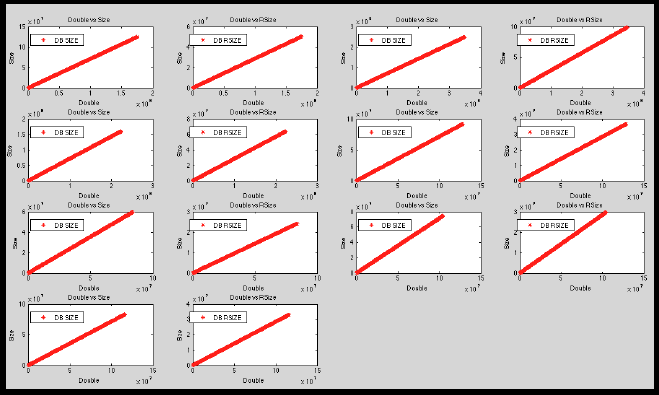
\includegraphics[scale=0.3]{sec.eps}\newline
				
					\textbf{Figure 19: Modified Database Scale}\newline
					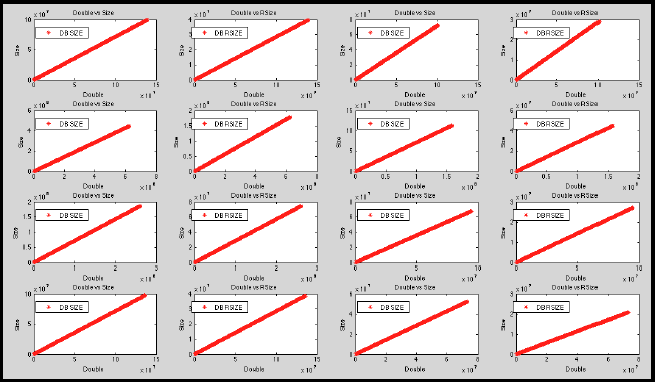
\includegraphics[scale=0.3]{fir.eps}		
		
  			\item[Cleaning] \hfill \\
  					In order to do this, we used the following MATLAB program that we coded 									specifically for our database, which has been attached to the report. \newline

					\textbf{Figure 20: Database Matlab Load File}\newline
					
\includegraphics[scale=0.35]{MCL1.eps}
				
					This part of the code loads all files from the location in dirList into names. Names 					contains a list of directories, and each one of these contains a list of data sets. 						In the for loop, each data set is being counted and weighted for comparison purpose. 					This code is run twice; the first time was ran on the normal database and its result 					is shown in Figure 18. The second time, it was ran on the modified database and its 						result is Figure 19. As you can observe, the first image has missing 	directories 							and datasets; that is how big it was, the software was not able to process it all. 						The second image has all directories and all datasets of each one, this is because 						the data is a lot smaller and it has shrink more than 30 percent of the normal data. 					The database has now been reduced to a 20 years old data.													\newline\newline\newline\newline\newline\newline\newline\newline\newline\newline\newline

					\textbf{Figure 21: Database Matlab Plot File}\newline
					
\includegraphics[scale=0.4]{MCL2.eps}
				
					This part of the code plots the size and the dataset number of each directory for 						comparison purpose. A quick hint to help to understand the image is by carefully 							looking at each one of the small graphs. If you notice, the  small graphs in the 							first figure have a higher range of those in the second figure. \newline

  					\textbf{Adding Meaningful Attributes}\newline 
						We have also coded a Java program to modify the datasets according to our 								design. For our design it was necessary to have the average temperature as well 						as a class that specifies a level of approximation as how cold or hot a place 							is. This would make it easier for us when applying normalization techniques to 							make datasets comparison much easier.\newline

						\textbf{Figure 22: Database Modificator JAVA Code}\newline
						
\includegraphics[scale=0.35]{JCL2.eps}
				
						This is a snip of the code and it contains the heart of the program. The first 							part of the program calculates the average temperature of a place. The maximum 							temperature is tp1 and the minimum temperature is tp2, then the average 									temperature is avgTemp is calculated by adding the two temperature and dividing 						it by 2. A very simple arithmetic function. The next step was to convert the 								actual temperature, as we all know the measurement in which we read the 									temperature in the USA is Fahrenheit. Therefore, we converted the actual 									temperature from Celsius to Fahrenheit to be able to make decisions easily 								without having to convert the value every time we access it.  After calculating 						the average temperature, and converting it from Celsius to Fahrenheit, we 								proceeded to create a ranking of how cold or hot a place is by analyzing its 								average temperature. The idea is to predict the weather trends of a place in a 							given future date, and therefore, the data must be prepared for classification. 						To facilitate temperature range predictions, we have created a derived 									attribute from the numeric minimum and maximum temperature attributes. The 								attribute HOC is derived as follows, by binning records based on which range 								their maximum and minimum temperatures falls into:\newline

						\begin{description}
  							\item[xx   to   38] \hfill \\
  								xx is considered as anything that is below 38F, and it is ranked as 										Very Cold or HOC = 0.
  							\item[39   to   58 ] \hfill \\
  								Anything between 39  F and 58  F is considered, in our table, as Cold 									or HOC = 1.
  							\item[59   to   68] \hfill \\
  								Anything between 59  F and 68  F is considered, in our table, as Cool 									or HOC = 2.
  							\item[69   to   77] \hfill \\
  								Anything between 69  F and 77  F is considered, in our table, as 											Comfort or HOC = 3.
  							\item[78   to   86] \hfill \\
  								Anything between 78  F and 86  F is considered, in our table, as Normal  								or HOC = 4.
   							\item[87   to   99] \hfill \\
  								Anything between 87  F and 99  F is considered, in our table, as Hot or 								HOC = 5.
  							\item[100 to 104] \hfill \\
  								Anything between 100F and 104F is considered, in our table, as Very Hot 								or HOC = 6.	
						\end{description}						

						This ranking will be very helpful when mining the data because we will not have 						to be looking at all temperatures and precipitation of the place. Instead, we 							will only have to check the ranking of this place to be able to give the user 							an advice in whether they should wear a coat or not.\newline

						\textbf{Creating an Mean Database}\newline
							We used R to load all datasets from all directories, which are exactly 									fifteen. We have extracted the mean value of each dataset for the 										temperatures obtained from 1980 to 2000. The results are very clear and 									self-explanatory, which can 	massively improve the mining algorithms 										implementation. The program that we 	have coded to create a mean database is 							shown below, and it is also attached to 	this project.  Also, we have 									created a confusion matrix for each one of the cities(directories) datasets 							to explain how this data representation can highly help during the mining 								and prediction process of this project. \newline

							\textbf{Figure 23: Mean Database R Code}\newline
							
\includegraphics[scale=0.4]{RCL1.eps}
			
							This is the code used to extract the mean values from each dataset in each 								directory. The variable "txt-files" contains all fifteen directories, then 								this is used to load the file into tables that R can read and extract the 								mean values from each one of its columns. There are some values that are 									not 	important, such as year and month. We are ignoring those in this case, 								our 	focus is in V8 and V9 the mean values of the average temperature and 									the 	weather ranking.\newline

							\textbf{Figure 24: Mean Database Rplot}\newline
							
\includegraphics[scale=0.35]{Rplot1.eps}
				
							This is the resulting confusion matrix from Alkansas-Red, one of the 										directories in our database, and the cities corresponding to this. As you 								can 	see, most of the weather temperature falls below 60 degrees F. This may 							not be 	as clear to you to read it because of the way the matrix is sorted. 							However, we 	have extracted important values from this matrix to explain 									below.\newline
				
							\textbf{Figure 25: Mean Dataset R-Histogram}\newline
							
\includegraphics[scale=0.35]{Rplot1-1.eps}
				
							We extracted two important variable from the dataset to analyze directly. 								These variables are V8 and V9, which are the average temperature and the 									ranking of the weather of the cities pertaining to the Alkansas-Red 										directory. Here it is more clear to observe what is going on in Alkansas-									Red during the years 1980 to 2000. You can see from 20 years of data, the 								most frequent temperature in this place is 60. They hardly got 70degrees F! 							Therefore, do not be surprised if our interface suggests you to wear a coat 							when planning to travel to this area.		
				
							\textbf{Figure 26: Mean Dataset R-Lineal}\newline
							
\includegraphics[scale=0.35]{Rplot1-12.eps}
				
							This image explains even better the weather situation in this place. As we 								observe, Alknsas-Red territory is not actually a bad place to travel to. 									For 	the most part is 60degrees F.  In winter the lowest it gets is 30, for 								the most part, and in summer the hottest it gets is 70. However, this is 									not a place to go to the beach! The weather here, according to our ranking, 							is for the most part comfortable. Therefore, cloths such as shorts and ten-								tops are not recommended for the most part.\newline
						
							We could have done the same analysis on the 15 territories, or directories, 							that we have in our database. However, we do not think this is necessary 									since it would take too much space out of our report. The analysis, based 								on the mean 	database, is very straight-forward. It avoid unnecessary 										analysis on our 	database, we can easily check in our database what 										probability does this territory has to be cold or hot before applying a 									more extensive analysis. Below are the images of the 15 territories, or 									directories, that provide a 	comparison of their average and ranking 										temperature.\newline
						
							\vspace{-3mm} 
							\textbf{Figure 27: Mean Database R-Lineal}\newline
							
\includegraphics[scale=0.3]{RCL15.eps}
				
							These are the graphs obtained from R that compares the average and ranking 								temperature of each territory or directory. Each graph represents a 										territory, or directory, and the weather datasets contains temperature only 							from 1980 to 2000.\newline
				
					\textbf{Creating a Zero-Database}\newline
						The data was filtered through our Java code to reduce our database to only 								20 years worth of weather data in all datasets of each city in our database. We 						have applied the Z-score technique to our database, but before this, we reduced 						the amount of data by removing some columns that are not important during the 							Z-score application process. For this we created another database in Matlab 								with important values from our normal database to apply the Z-score technique. 							As a result, we created another database based on the results obtained from the 						important values database after applying the Z-score technique. Finally, we 								compared results from the normal database, important values database, and Z-								score database by comparing the first set of the last territory of each 									database to make testing easier and more efficient. Below is the program, 								divided in parts, that we have coded in Matlab, and a detailed description of 							each part of this code.\newline 

						\textbf{Figure 28:Database Matlab Load File}\newline
						
\includegraphics[scale=0.35]{MZCL1.eps}
				
				 		In this part of the code, we are accessing all the sub-directories, or 									territories, and saving them in the variable "tf." Then, we count the number of 						sub-directories and save this in the variable "numberOfFolders" to use in 								further analysis of this code. This part of the code only focuses in accessing 							and counting all of the territories in our database.\newline
				 
				 		\textbf{Figure 29:Database-1Dataset Matrixplot Code}\newline
						
\includegraphics[scale=0.4]{MZCL2.eps}
				
						The first loop in this code is to analyze the current data. Remember that the 							current data in our database is not as dirty as it was before. We have already 							removed unnecessary data and added important attributes that  make our datasets 						more meaningful in our database  to make data analysis and mining easier and 								faster. In this part of the code we are accessing all sub-directories and, once 						in the subdirectory, we are accessing all datasets or text files and saving 								them into the variable "fid."  For our data analysis we only loaded one file, 							the first dataset, to make the analysis and comparison of the data easier. 								However, to create the Zero database this code was modified by only adding a 								loop inside this part of the code. In this way, we load all text files, or 								datasets, into the variable s and then add this to our list of subdirectories 							"A." Inside the loop we plot the first dataset of each sub-directory , for best 						results and comparison purpose we used the confusion matrix plot from Matlab. 							Outside the loop we plot the last subdirectory, folder 15, just to better 								explain users what is exactly happening with the data. Since we put all 15 								plots together in one figure it may be difficult for users to relate to the 								data, and therefore, we decided to plot one of the sub-directory dataset and 								explain it in details.\newline
						
						\textbf{Figure 30:Database-1Dataset Boxplot Code}\newline
						
\includegraphics[scale=0.5]{MZCL3.eps}
								
						After using the confusion matrix from Matlab, to better analyze the data and to 						explain its behavior in relation to our interface, we decided to use another 								plotting type from Matlab. The plot type that we used was the boxplot, and 								gives a complete different view of the weather data contained in the data sets 							of multiple territories or directories.\newline
				 
				 		\textbf{Figure 31:Database Modification}\newline
						
\includegraphics[scale=0.45]{MZCL4.eps}
								 
				 		The analysis performed above was only about our normal database, which contains 						years, month, max and min temperature, precipitation, wind speed, average 								temperature in Celsius, average temperature in Fahrenheit, and ranking 									temperature. We came to the conclusion that in order to make a better analysis 							of this database we need to clean it even more, which means creating another 								database that contains only the important or meaningful attributes for a deeper 						analysis of the data. For example, if a user is looking for cloth wearing 								suggestions to travel to certain place in certain date. If we happen to be in 							winter, and according to our database deeper analysis, this place is cold 								95 percent of the time. Then,there is no point to search and analyse 20 years 							worth of data. This is why we thought of this and the R database to make 									suggestions and 	weather trends prediction faster and easier. The system can 								easily access this database, to avoid a longer and slower analysis, and have a 							fast respond on 	whether this person needs a coat or not. We decided that 									minimum and maximum 	temperature, precipitation, wind speed, and average 									temperature in Fahrenheit were the most important an more meaningful attributes 						for this database. The way we created this database was through Matlab, by 								extracting the important attributes from our current database into a new 									database. This is exactly what the code in Figure 32 is doing, is moving 									columns 3, 4, 5, 6, and 8 from A(our current database) to columns 1, 2, 3, 4, 							and 5 from B(our new database.)\newline		

						\textbf{Figure 32:Zero Database Process 1}\newline
						
\includegraphics[scale=0.45]{MZCL5-1.eps}
								
						In order to make better use of the weather data provided by our database, it 								was necessary for us to make some modifications to lead us to a better 									interpretation of the data. As we explained before, our weather data is based 							on the year, month, precipitation, max and min temperature, and we have added 							the average temperature, and temperature scale parameters. These attributes 								allow us to mine the data faster and more efficient, especially the temperature 						scale parameters which actually approximates the comfort level of the 									temperature. Also, we have created three databases, the normal, R, and  new 								database, to help improving the data analysis and mining of our system. The 								next step is to create a Z-score database, Matlab made it easy for us to do 								this step. Since we had already extracted the most important attributes from 								our database, it was easy for us to just apply the Z-score method on the new 								database and save the results on to a third database that contains all the Z-								score values of the weather data of all territories or directories of our 								database. Furthermore, we decided to record the mean and standard deviation 								values of each dataset along with their Z-score values of the attributes 									previously mentioned when creating the new database.\newline
				
						\textbf{Figure 33:Zero Database Process 2}\newline
						
\includegraphics[scale=0.45]{MZCL5-2.eps}
				
						This is the code that we used to record the mean value of each column, or 								attributes previously mentioned when creating the new database, on each data 								set contained in each directory or territory. \newline
						
						\textbf{Figure 34:Zero Database Process 3}\newline
						
\includegraphics[scale=0.45]{MZCL5-3.eps}
								
						This is the code that we used to record the Z-score value of each row, of all 							attributes previously mentioned when creating the new database, on each data 								set contained in each directory or territory. \newline

						\textbf{Figure 35:Zero Database Process 4}\newline
						
\includegraphics[scale=0.45]{MZCL5-4.eps}

						This is the code that we used to record the  standard deviation value of each 							column, or attributes previously mentioned when creating the new database, on 							each data set contained in each directory or territory. \newline

						\textbf{Figure 36:ZDB Process 5 - Matrix Plot}\newline
						
\includegraphics[scale=0.45]{MZCL5-5.eps}
								
						Finally, we proceeded to plot one dataset of each directory or territory for 								analysis and comparison purpose. As you can see, just like in the other loops, 							we have individually plot territory 15 from our Z-score database to help users 							to relate to the data.  We used the confusion matrix plot from Matlab.\newline
				
						\textbf{Figure 37:Zero Database Boxplot}\newline
						
\includegraphics[scale=0.45]{MZCL6.eps}

						This part of the code was used to graph the data just as in the above code, the 						only difference is that we are using box plotting instead. This helps us to 								better understand the analysis from a different point of view. \newline

						\textbf{Figure 38:New Database Box Plot}\newline
						
\includegraphics[scale=0.45]{MZCL7.eps}
						
						\textbf{Figure 39:New Database Matrix Plot}\newline	
						
\includegraphics[scale=0.45]{MZCL8.eps}
						
						Since we already graphed the normal and Z-score database, we have decided to 								graph the new database as well. The code you see in Figure 38 is the code to 								graph the first data set of all directories in a box plot from Matlab. In a 								similar way, the code in Figure 39 is to graph the first data set of all 									directories in the new database in matrix plot. Graphing is very important in 							this case to make users understand the difference between each database and 								their importance in our system. Also to help users understand the effect of 								each technique on each database and our system. We proceeded to compare and 								analysis each one of these figures in the following manner.\newline			
				
					\textbf{Normal Database Data Analysis}\newline
						\textbf{Figure 40:Normal Database Matrix Plot}\newline
						\hbox{\hspace{-9ex}
\includegraphics[scale=0.27]{MCNM-AllA-All.eps}}
						These graphs are a result from some of the code explained above. We are 									analyzing and comparing each one of the graphs so this way users can have a 								better understanding of the  data, and can relate to each technique and result. 						We first plotted the first data set from each one of the territory in our 								normal database, which are 15 directories and as you can see in the image there 						are 15 plots. The normal database is composed of the year, month, minimum and 							maximum temperature, precipitation, wind speed, average temperature in Celsius, 						average temperature in Fahrenheit, and ranking temperature. Nevertheless, we 								only plotted the year, month, average temperature in Fahrenheit, and the 									ranking temperature. Since the image in Figure 40 is not to clear we will 								proceed to explain one of the datasets from the directory 15, which is also 								included Figure 40. \newpage
						
						\textbf{Figure 41:Normal Dataset Matrix Plot}\newline
						\hbox{\hspace{-10ex}
\includegraphics[scale=0.27]{MCNM-15A-1.eps}}		
						This Figure 41 explains a better the behavior of the data. During the years of 							1980, 1985, 1990, and 2000 the temperature average was of about 80 degrees 								Fahrenheit. The highest ranking  for the years 1984-5, 1989, 1991-2, 1994, 1996 						and 2000 was of 3, and for the rest of the years it was 4. This means that out 							of 20 years this place has reached the level 4th 13 times, which means that 								this place has on average a normal temperature ranging from 78 to 86 degrees 								Fahrenheit. The lower block to the right shows the months that have been the 								hottest. We easily see how from May to August the temperature reaches its 								hottest, and in this case the hottest is below 86 within the normal 										temperature. From April to November temperatures reaches a comfortable level, 							the 3rd level for the most part, ranging from 68 to 77 with the possibility 								of reaching level 4th . This is all the information we were able to obtain from 						the normal database, which was easy to predict due to the ranking temperature 							variable. However, we are hoping that the other implementations, or databases, 							reduce the data amount and analysis time when mining.\newline	
							
						\textbf{Figure 42:Normal Database Box Plot}\newline
						\hbox{\hspace{-8ex}
\includegraphics[scale=0.27]{MCNM_AllB_All.eps}}		
						This Figure 42 is a different plot, or boxplot, from Matlab. We decided 									to graph it in this format with the hope of better understand the data and 								maybe to get better results. As in the previous Figure, this image contains 15 							plots that contain the weather data from the 15 directories or territories in 							our normal database. A better explanation of the boxplot and weather data is 								given in Figure 43, by analyzing one of the plot shown in the current 									Figure 42.\newline
					
						\textbf{Figure 43:Normal Dataset Box Plot}\newline
						\hbox{\hspace{-10ex}
\includegraphics[scale=0.27]{MCNM-15B-1.eps}}			
						In this plot we are analyzing more data than in the matrixplot. We are 									analyzing columns 3, 4, 5, 6, 7, 8, and 9, which are minimum and maximum 									temperature, wind speed, average temperature Celsius and Fahrenheit,  and 								ranking temperature. This is the same dataset as in the matrixplot, first data 							set from the directory  or territory 15. Honestly, I did not like the output 								from boxplot. However, the answer is understandable since we fed the box with 							too 	much data. Even though the output is not as informative as in the previous 							one, we still are able to make some smart assumptions based on the data. The 								first bucket, which is the one to the left, contains the temperature that this 							place often phased. The temperature of this place is in normal level, level 4th  						since it ranges from more than 50 to less than 90 degrees Fahrenheit.\newline 	
				
					\textbf{Unique Values Database Data Analysis}\newline\newline
						\textbf{Figure 44:New Database Matrix Plot}\newline
						\hbox{\hspace{-7ex}\includegraphics[scale=0.27]{MCBM-AllA-All.eps}}				
						The same procedure that was taken to graph a plot of each one of directory in 							the normal database was taken to graph the plots of the first data set of each 							territory in the new database. The new database is composed by unique values 								that are important to our system and could make data analysis and mining easier 						and faster. These values are minimum and maximum temperature, average, 									precipitation, wind speed, and average temperature in Fahrenheit. In the same 							way as in the previous database analysis, we will explain in detail the 									analysis of this database by analyzing one of the data sets from one of the 								plots in this Figure 44.\newpage		
						
						\textbf{Figure 45:New Dataset Matrix Plot}\newline
						\hbox{\hspace{-8ex}\includegraphics[scale=0.25]{MCBM-15A-1.eps}}					
						This graph is plotting all of the attributes of the new database, which were 								mentioned above. Even though this database only contains important attributes 							of our system, it is not very useful all on its own. From Figure 45 all you 								can get is that temperatures during those 20 years ranged between about 45 and 							85 degrees, everything else is irrelevant and does not add any meaning to the 							data. The good thing about this database is that makes it easy for to create a 							Z-score database. Also, this database is of great use when combining with the 							results obtained in the R-database.
				
						\textbf{Figure 46:New Database Box Plot}\newline
						\hbox{\hspace{-6ex}
\includegraphics[scale=0.25]{MCBM-AllB-All.eps}}				
						We decided to graph it in this format with the hope of understanding better the 						data, and maybe getting better results. As in the image above, Figure 46 									contains 15 plots that contain the weather data from the 15 directories or 								territories in our normal database. A better explanation of the boxplot and 								weather data is given in Figure 47, by analyzing one of the plot shown in the 							current Figure 46.
				
						\textbf{Figure 47:New Dataset Box Plot}\newline
						\hbox{\hspace{-7ex}\includegraphics[scale=0.25]{MCBM-15B-1.eps}}	
										
						This plot is just as useless as the plot above. We do not get much information 							from it, only the fact that most of the temperature during those 20 years of 								weather data ranges from 77 to 86. Therefore, falling within the normal level 							of temperature in the USA temperature system.\newline
				
					\textbf{Z-score Database}\newline				
						\textbf{Figure 48:Z-score Database Matrix Plot}\newline
						\hbox{\hspace{-9ex}
\includegraphics[scale=0.27]{MCZM-AllA-All.eps}}				
						This is the last database that we created, hoping to get better results 									than in the new database. The attributes of this database are the same as those 						mentioned in the new database, or unique values database. The only difference 							is that we have applied the Z-score method to each one of the attributes, 								hoping for a better result during data analysis to facilitate data mining. As 							we mentioned in the other database analysis, a better explanation of the matrix 						plot is given by choosing one of the data sets from one of the 15 directories							    plotted in Figure 48. \newline
			
						\textbf{Figure 49:Z-score Database Matrix Plot}\newline
						\hbox{\hspace{-9ex}
\includegraphics[scale=0.27]{MCZM-15A-1.eps}}	
						As we can observe in the image the plot has improve a lot. We have reduced the 							data to its maximum and it is less confusing. It is easier to make assumptions 							from this plot and use it for analysis purpose. The average temperature can be 							used as the ranking number that we used, if you see, the average temperature is 						below 5, just as we predicted. The max, min, precipitation, and win speed is 								also centered, which means that this place is with the normal level of the 								temperature. Z-score can easily explain the behavior of the data set, if in 								this place it was cold for the most part it would show the data distribution on 						the 	left side of the scale, and opposite if it was hot for the most part. 								However, since most of the temperatures were within the normal level the data 							distribution this is centered. This means, if a person were planning to 									travel in summer to this place I would suggest to wear normal clothing as well 							as short since 68F – 77F it is a good temperature to wear shorts at least in 								the afternoon.\newline
				
						\textbf{Figure 50:Z-score Database Box Plot}\newline
						\hbox{\hspace{-9ex}
\includegraphics[scale=0.27]{MCZM-AllB-All.eps}}
						We decided to use Box plot format with the hope of understanding better the 								data, and maybe getting better results than that obtained during the new 									database analysis. As in the image above, Figure 50 contains 15 plots that 								contain the weather data from 15 directories or territories in our normal 								database. A better explanation of the boxplot and weather data is given in the 							Figure 51, by analyzing one of the plots shown in the current Figure 50.									\newline
				
						\textbf{Figure 51:Z-score Dataset Box Plot}\newline
						\hbox{\hspace{-10ex}
\includegraphics[scale=0.27]{MCZM-15B-1.eps}}				
						This Figure 51 is better than the one obtained in the new database analysis. 								Here we observe a better behavior of the data. It is easy to see how centered 							the data is, and make assumptions from it. As we can see, most of the 									temperatures are within the 3rd level. This is actually the first analysis in 							which the boxplot shows better results than the matrixplot, and this is because 						of the Z-score method. Figure 51 shows how most temperatures reach the 3rd 								level, but some temperatures get to the 4th level or even above but below 5. It 						also shows how 	all temperatures are within a normal range, the lines in read,  						for the most part the weather is within normal temperatures of 68F-77F 									(comfortable temperature), but it can reach temperatures of 77F-86F (normal 								temperature) during summer.\newline 

					As a result, we have created four databases to improve data analysis and mining. It 						was very clear that our normal database, obtained by cleaning the real database, is 						of great use the way it is. However, to improve the efficiency of our system we 							decided to play a bit more with the database and create more databases that could be 					of great use during mining. The new database results are not very helpful by itself, 					it needs other factors such as the R-database, which contain the mean values of all 						datasets. On the other hand, the creation of the new database made it easy for us to 					create the Z-score database. The Z-score database can be used along with the new 							database to avoid further and extensive analysis of the data when suggesting the 							user what to wear when travelling. Z-score method reduce a lot of the data and 							summarize in a way that is much easier for a person and our system to understand 							when making a decision or prediction.\newline 
					
		\end{description}
		
	
	\subsection*{Interface}
	
		The data will be used to predict the weather for future dates by analyzing weather in the past. 			In order to achieve this we are making use of the k-nearest-neighbor algorithm. The idea is to 			use this knowledge discovery technique to predict weather trends from the weather data in our 			database. We will be comparing similar weather situations to 	predict what the percentage of 				precipitation would be, given certain conditions. We plan to 	adapt this approach to approximate 			the 	range for minimum and maximum temperatures, and give user cloth wearing suggestions.\newline 

		\textbf{Data Access} \newline
			\textbf{Figure 52:Actual Interface Implementation}\newline
			
\includegraphics[scale=0.25]{imp1.eps}		
		
			In order for users to perform any kind of task, users need to access our system through our 				website. Once in, we get access to the necessary information, input by the user, to proceed 				with the search and provide users with a cloth wearing suggestion. Webapp2 easily connects 				python to our domain in order to process the necessary information for any given query.					\newpage
		
			\textbf{Figure 53:Search Implementation}\newline
			
\includegraphics[scale=0.5]{imp2.eps}
		
			In this feature we are searching into our database through webapp2 for a particular city, 				but 	since DJango is not completely setup we are using an alternative engine software 						explained below. Anyway, this is done by entering the city name that queries into the 					database class. The alternate app application is not as efficient as the DJango application, 			but 	could be easily linked to DJango platform in a future.\newline

			Graph:\newline
				The graph is generated through the function that we have built into the application 						engine. This takes take the regression of the data of each day within a given range. 						Then, we use the graph with the resulting data using python, and resulting data is an 					approximation of the weather that the user has selected for travelling purpose, an 						example of this function is in Figure 23.\newline

			Suggested List:\newline
				This has not been implemented in our interface yet. However, our system is design so 						every time the user searches for a city this search is being saved by webapp2 in a 						separate table. Also, it stores the average temperature of the queried destination.  We 					query into our database using the average temperature to suggest the user with a list of 				appropriate destinations in a future. \newline	

		\textbf{Alternative Interface Application}\newline
			We have implemented a RESTful web service in Python using the webapp2 framework, hosted on 				Google's App Engine platform. The service leverages the schema-less NDB datastore provided 				by App Engine, and relies on the underlying App Engine platform to scale both the datastore 				and number of running application instances automatically based on load. The service takes a 			user-supplied latitude, longitude and date and returns a prediction for the average weather 				for that month, computed using the method in the next section, to the user.\newline

			Although the datastore is schema-less, we have created a simple format for storing time-					series data points for monthly averages of weather data, including monthly precipitation, 				average high and low temperatures, and average wind speed. We chose to store monthly data 				instead of daily data due to limitations of the free tier of service of App Engine, which 				imposes limits on how many writes can be performed on the datastore, and the raw amount of 				data that can be stored. As stated earlier, we have also chosen to limit the data stored to 				instances ranging from 1980 to 2000, again due to storage limitations. In addition, we have 				decided to use only the data from the Great Lakes "basin" for data mining. This limits the 				area for which predictions can be made to the area surrounding the great lakes in the 					north-eastern United States and Canada.\newline

		\textbf{Data Mining}\newline

			To predict the weather for a given month (within the range that data is available), we use a 			modified version of the k-nearest neighbors algorithm. This algorithm classifies based on 				the k nearest instances in it is training set to a given instance. The "closeness" of 					instances is measured by some distance metric defined on the space of feature vectors of the 			data. In our data, we define a data point's feature as a vector that is defined as the set 				of its numerical attributes, excluding the time-series attributes (i.e. temperature, 						precipitation and wind speed).\newline

 			A user of the web service makes a query for a given month, year, latitude and longitude. The 			web service then identifies four corners of a grid cell for which data is available; the 					cell being the quadrilateral region in which the user-supplied latitude and longitude falls. 			Once this cell is established, the ten nearest neighboring points for each corner for the 				month previous to the one supplied by the user. These points are chosen based on the 						unweighed Euclidean distance between the feature vectors of each point and the corner point 				of the cell. Once the ten nearest neighbors are retrieved, they are replaced by the 						instances for the same location but one month later. The reason for selecting the neighbors 				in this manner is because we expect that we can find a month in the past that was "like" 					last month, we can predict the weather for this month (or next month) by looking at the 					following month in the past. \newline

			The average of the ten neighbors' numerical weather values are taken for each corner, and 				then the predicted values are taken to be the average of the predictions for the four 					corners of the cell. We believe this is a reasonable approximation, as the cells are small 				(1/8 degree latitude and longitude), and the weather doesn't tend to change much over small 				areas. \newline

		\textbf{Testing}\newline

			To test the accuracy of this service, we will select a random subset of the data from the 				last year available (2000), and compare predicted values for the selected instances to their 			known values. At the time of this writing, we do not have results for this testing, as the 				tests are currently executing. The tests are somewhat computationally expensive, mostly due 				to the volume of the data and certain limitations in the manner in which data may be queried 			from the schema-less NDB datastore.\newline

		These components were planned, analyzed, and designed into our system through documentation 				such as data flow diagrams and others that will guide users to use our system if any issue 				arises. We have tested our system several times to make sure that our system works and 					performs the duties it is intended to perform. It was critical to make sure that each 					application was implemented in accordance with our design and architecture plan to ensure 				that our system is ready for implementation. In this way, we were able to determine issues, 				occurred during the implementation process, which affected our system. Overall, we have 					established an overall development with the best practices to achieve the goal of our system 				implementation.	\newline	
		
\section{Lessons Learned}
	\label{Lessons Learned}
	
	We learned numerous cleaning and mining techniques while working on this project. We learned a 			number of ways of preparing our data so that we can easily use it in our application. For example, 		the data downloaded from the website was raw and faulty, we added average temperature, Fahrenheit 		temperature, and ranking temperature to each data set to make it more meaningful. We also learned 		how to convert text less into mysql database so as to be able to use in our project.\newline

	We learned how to clean a database to make query easy on a huge database. As a result of querying 		for the weather conditions of a place, we get a number of results by using regression techniques on 		our database. This provides a single ranking value for each corresponding date that the user is 			going to be on vacation.\newline

	We also learned a few data mining techniques that we were not able to include in our interface 			because we ran out of time. We are currently able to suggest a few vacation destinations for our 			users, but in order to provide users with such information we need to make our application more 			interactive. The suggestions are based on the age, gender and the last search made by the user. 			Using these variables it is easy to perform data mining, as mentioned above, to search in our 			database for more destinations that the user may like.\newline

\section{Current Status}
	\label{current status}
	
	The current status of our project is being explained through the three main sections that gave place 	to our project development.\newline

	First, we gathered the weather data of a few cities of U.S.A. This data consists of temperature, 			precipitation and wind speed corresponding to each city from 1980 to 2000. Each city is related to 		an id, latitude, and longitude. \newline

	Second, we developed an interface to provide the user with a GUI to query efficiently on the 				database. The interface allow the users to search for destinations to vacation in a given range of 		dates. There is no log on, which allows the user to avoid the whole process of signing in. The users 	can choose a place from this list, or search for their city of preference to vacation, and the 			vacation time duration. Then, the application searches for the corresponding weather data of the 			place and approximate temperature, precipitation, and wind speed of the place to suggest an adequate 	cloth to wear. \newline

	Lastly, the suggested cities, which is not incorporated on interface yet, before and after the user 		search is done we use a data mining technique known as association rule discovery. In this way, we 		can provide users with list of suggested cities and make our interface more interactive.\newline

\section{Future Status}
	\label{Future status}
	\begin{itemize}
		\item[] Big Data:\newline
			More research is needed to improve the ability to blend different datasets, and data sources 			into integrated systems. As new types, data could be assimilated into different models. 					Also, it will be important to understand the error characteristics of our current data and 				our model to come up with modifications that may improve our system. Data assimilation for 				climate purposes is still in an early stage of development and requires continued research 				support. As these developments occur, reprocessing of data to take advantage of the new 					knowledge will be vital if we want to sustain long-term records in the future.\newline
		
		\item[] Data Mining:\newline
			If our weather observations were well-documented, and it contained good metadata about the 				systems and networks used to make them, it would become more valuable with time. The 						creation of weather-quality data records is a fundamental objective for our observing system 			for weather. International standards and procedures for the storage and exchange of metadata 			need to be developed and implemented for many weather observing system components, including 			those of the operational satellite community. For this, it will be essential that all such 				data be properly archived and managed with the full expectation that they will be reused 					many times over in the future, often as a part of reprocessing or reanalysis activities. 					Future modifications may require that data be migrated to new media as technology changes, 				be accessible to users, and be made available with minimal incremental costs. For this, we 				will need systems for quality control and feedback, proper data archival and access, 						sustained data preservation, rescue and digitization, and climate data management 						systems\newpage
			
	\end{itemize}

\section{Conclusion}
	\label{Conclusion}
	
	This project, "What Should I Wear," was prepared in response to avoid travelling unprepared when an 		unexpected bad weather hits during a vacation trip. The full implementation of the project, over the 	coming years, will ensure users to have the observational information needed to understand, predict, 	and manage their response to weather and weather change, over the 21st century and beyond, for 			vacation purposes. It will address the commitments of the users to certain places, and support 			their needs for weather observations in fulfilment of the objectives of their vacation. The 				database sustains observations of the essential climate variables that are used to make significant 		progress in the generation of weather analysis and derived information for our project. These 			observations give an enhanced support to our research, modelling, and analysis for users' s cloth 		wearing in any event. In fact, these observational records improve weather predictions for short-			term travelling, especially vacations. These observations must be sustained into the future to 			evaluate how the weather is changing so that informed decisions can be made by any user on 				prevention, mitigation, and strategies when travelling. It is crucial for users to support the 			further research needed to refine understanding of the approximated weather and its changes. This 		will allows us to initialize predictions on time scales out to decades ahead, and to develop the 			models used to make these predictions as well as short-term scenario-based projections.

\section{References}

	[1] NCDC. Babel, Whether Datasets. cdo-web,
		12(2):291-301, June 1991.
		http://www.ncdc.noaa.gov/cdo-web/
		\newline

	[2] M. Clark. Post congress tristesse. In TeX90 Conference
		Proceedings, pages 84-89. TeX Users Group, March1991.
		\newline

	[3] M. Herlihy. A methodology for implementing highly
		concurrent data objects. ACM Trans. Program. Lang.
		Syst., 15(5):745-770, November 1993.
		\newline

\end{document}